\documentclass{article}%
\usepackage[T1]{fontenc}%
\usepackage[utf8]{inputenc}%
\usepackage{lmodern}%
\usepackage{textcomp}%
\usepackage{lastpage}%
\usepackage{authblk}%
\usepackage{graphicx}%
%
\title{Dual Inhibiting Senescence and Epithelial{-}to{-}Mesenchymal Transition by Erythropoietin Preserve Tubular Epithelial Cell Regeneration and Ameliorate Renal Fibrosis in Unilateral Ureteral Obstruction}%
\author{Michael Ramsey}%
\affil{Department of Oral and Maxillofacial Surgery, Hyogo College of Medicine, Nishinomiya, Hyogo 663{-}8501, Japan, Department of Genetics, Hyogo College of Medicine, Nishinomiya, Hyogo 663{-}8501, Japan}%
\date{01{-}01{-}2013}%
%
\begin{document}%
\normalsize%
\maketitle%
\section{Abstract}%
\label{sec:Abstract}%
SAN DIEGO (KGTV) {-} The use of sequence transfection protein to achieve biologic infection{-}fighting immunity is a new and novel approach to achieving endovascular clearance of Adenoviruses (Auerent) and Microbes that are a known nuisance in vascular pathways such as circulation and retinal blood flow.\newline%
Genesis Cell Therapeutics is a privately held company developing therapies to eliminate Auerent{-}like interneurons and microorganisms or host to them. However, the cells have made it difficult to enter the vascular endothelial cells of human patients, which could limit the potential for eventual immunological remediation. Genesis Cell has derived an approach that can circumvent such factors.\newline%
This work was funded by the Clinical Research Network (CRI) program under the U.S. Department of Veterans Affairs Office of Research and Development. The work was supported by funds from the National Institutes of Health (NIH) and from data and data disclosures from the VES and VES Biopsies. The ves included 13 confirmed clinical studies of gene expression in vascular endothelial cells after delivery of mRNA to the endothelial cells. These studies have since been published in some of the largest journals on biology of vascular endothelial function and clinical disease.

%
\subsection{Image Analysis}%
\label{subsec:ImageAnalysis}%


\begin{figure}[h!]%
\centering%
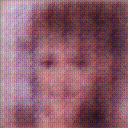
\includegraphics[width=150px]{500_fake_images/samples_5_168.png}%
\caption{A Close Up Of A Person Wearing A Suit And Tie}%
\end{figure}

%
\end{document}